\subsection{SP-5 (DBS)}
Relační databáze, dotazování v relační algebře, základní koncepce jazyka SQL (SELECT, DDL, DML, DCL, TCL), vyjádření integritních omezení v DDL.

\subsubsection*{Relační databáze}
\begin{itemize}
	\item databáze je soubor záznamů, jejichž systematická struktura umožňuje, aby tyto zprávy mohly být vyhledávány pomocí počítače
	\item existence dat v DB je nezávislá na aplikačních programech
	\item zabývá se řízením velkého množství, perzistentních, spolehlivých a sdílených dat
	\begin{itemize}
		\item velké množství --- nestačí operační paměť
		\item perzistentní --- data přetrvávají od zpracování ke zpracování
		\item spolehlivá --- lze rekonstruovat po chybě
		\item sdílená --- přístupná více uživatelům
	\end{itemize}
	\item hlavní přínosy DB technologií:
	\begin{itemize}
		\item nezávislost dat na aplikaci
		\item efektivní přístup k datům
		\item urychlení vývoje aplikací
		\item integrita a ochrana dat
		\item správa a zálohování dat
		\item transakční zpracování
		\item paralelní přístup k datům
		\item zotavení po chybě
	\end{itemize}
	\item DBS --- Database system
	\item DBMS --- Database Management system
	\item relace --- dvourozměrná struktura (tabulka)
	\begin{itemize}
		\item atributy (sloupce) --- jména a domény atributů
		\item n-tice (řádky) --- prvky relace (unikátní)
	\end{itemize}
	\item schéma relační databáze: množina relací $R$ a množina integritních omezení $I$
\end{itemize}

\subsubsection*{Relační algebra}
\begin{itemize}
	\item pouze dotazovací formalismus (vyhledávání dat)
	\item specifikujeme co chceme, ne jak to získat
	\item výsledkem dotazu je relace (lze použít pro další dotaz)
	\item jakýkoliv jazyk realizující relační algebru se nazývá relačně úplný
	\item dotazování:
	\begin{itemize}
		\item nazev\_relace(''atribut'' = hodnota) --- vyhledání záznamů v dané relaci, které vyhovují podmínce (pod\-mín\-ka není nutná) --- tento proces se nazývá selekce 
		\item nazev\_relace(podminka)[atribut1, atribut2] --- hranaté závorky jsou výběr atributů, které se vloží do výsledné relace --- nazýváme projekce
		\item relace1 * relace2 --- přirozené spojení relací na základě stejně se jmenujících atributů
		\item nazev\_relace[atribut1 $\rightarrow$ jine\_jmeno]
		\item množinové operace jako sjednocení, průnik, rozdíl a kartézský součin ($\cup$, $\cap$, $\setminus$, $\times$)
		\item polospojení (left/right join) relace1 *$>$ relace2
	\end{itemize}
\end{itemize}

\subsubsection*{SQL}
\begin{itemize}
	\item Structured Query Language
	\item relačně úplný (jakýkoliv dotaz v RA lze převést do SQL)
	\item podobně jako u RA řešíme jaký chceme výsledek, ne jakým způsobem ho získat
	\item části SQL:
	\begin{itemize}
		\item DDL (Data Definition Language) --- create, alter, drop (tvorba relací samotných, také řeší integritní omezení)
		\item DML (Data Modification Language) --- insert, update, delete, merge, transakční zpracování (úprava záznamů v relacích / tabulkách)
		\item DCL (Data Control Language) --- grant, revoke (úprava práv uživatelů, přístupy)
		\item TCL (Transaction Control Language) --- commit, rollback, savepoint
	\end{itemize}
\end{itemize}

\subsubsection*{Integritní omezení}
\begin{itemize}
	\item realizované pomocí DDL
	\item můžou se kontrolovat periodicky či při každé úpravě
	\item 2 typy omezení:
	\begin{itemize}
		\item deklarativní (pro domény atributů) --- kontrola hodnoty samotných atributů, např. nesmí být nějaké hodnoty (NOT NULL, CHECK) nebo další omezení (UNIQUE, PRIMARY KEY, FOREIGN KEY / REFERENCES)
		\item procedurální (složitější) --- nad celými tabulkami, trigger
	\end{itemize}
	\item vyjádření integritních omezení v příkazu CREATE:
	
	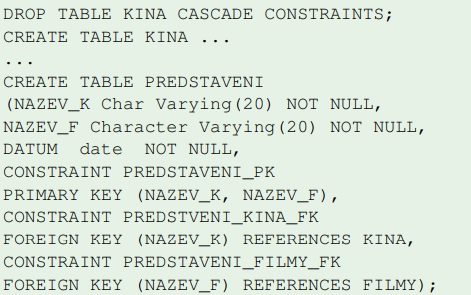
\includegraphics[width=0.7\textwidth]{img/SP-5_0.jpg}
\end{itemize}